\documentclass[10pt,reqno]{amsart}
\usepackage{articlesetup}
\usepackage{float}

\bibliography{bibliography}

\author{Harvey J. Stein}
\email{hjstein@bloomberg.net}

\date{\today}

\begin{document}

\title{COVID-19 data collection: Garbage In, Garbage Out}

\begin{abstract}
  COVID-19 data discussion.
\end{abstract}

\maketitle
\tableofcontents

\section{Introduction}
\label{sec:intro}
If you recall my 4/21 analysis of the NYC COVID-19 data
(\href{https://hjstein.blogspot.com/2020/04/covid-19-nyc-stats-not-what-they-seem.html}{COVID-19 NYC Stats -- Not What They Seem}),
you'd remember a graph showing the extent to which missing
data has a major impact on the reported incident
counts.\nocite{nyc2020data,Stein2020nycdata,Stein2020owiddata,owid2020data}
Figure~\ref{fig:daily} has an updated version.\nocite{Stein2020Seem}\nocite{Stein2020Ray}

\begin{figure}[H]
  \centering
  \includegraphics[width=\textwidth]{../Notebooks/casesPerDayHistoryRaw.png}
  \caption{NYC COVID-19 cases per day from each daily report.  Data
    from the NYC COVID-19 data github repository.}
  \label{fig:daily}
\end{figure}

As you can see, the peak hasn't moved from April 7th, but we're still
getting data for dates as far back as March!
Figure~\ref{fig:smoothDaily} has the updated 7 day average report,
which shows more clearly that three days ago additional incidents were
reported for every date going back as far as March 25th.

\begin{figure}[H]
  \centering
  \includegraphics[width=\textwidth]{../Notebooks/casesPerDayHistory.png}
  \caption{7-day rolling average of NYC COVID-19 cases per day from each daily report.  Data
    from the NYC COVID-19 data github repository.}
  \label{fig:smoothDaily}
\end{figure}

After seeing this analysis, Jon Asmundsson, editor of {\it Bloomberg
  Markets} asked me if this holds for other regions.\cite{Asmundsson2020Dates}
%% \begin{quotation}
%%   Your analysis is really interesting.  Have you looked at other states/cities?
%% \end{quotation}

This led me to try.

\section{Garbage in}
My first stop was the
\href{https://github.com/owid/covid-19-data}{Our World in Data github
  repository}\nocite{owid2020data}.  I
\href{https://github.com/hjstein/covid-19-data}{forked the
  repository}, imported my analysis code, extracted the historical
reports and graphed the history.  The results are in figure~\ref{fig:owid}.

\begin{figure}[H]
  \centering
  \includegraphics[width=\textwidth]{../../covid-19-data/scripts/notebooks/casesPerDayHistory.png}
  \caption{USA COVID-19 cases per day from each daily report.  Data
    from the OWID COVID-19 data github repository.}
  \label{fig:owid}
\end{figure}

It's nice that the 7 day average is dropping, but where are the new
reports?  There are no updates -- no missing data!  How could it be
that the data the USA cases counts for yesterday that they receive
today are complete?  Given what we know about the NYC data, and given
that the NYC data is part of the USA data, it can't possibly be the
case that on a given day they know exactly the number of cases the day
before.  Something odd must be going on.

So I entered an
\href{https://github.com/owid/covid-19-data/issues/41}{issue on the
  OWID COVID-19 github repository}.  I asked how they generate the
data.  Edouard Mathieu, Data Manager at OWID, responded:
\begin{quotation}
  For confirmed cases and deaths, our data comes from the European
  Centre for Disease Prevention and Control (ECDC). We discuss how and
  when the ECDC collects and publishes this data \href{https://ourworldindata.org/coronavirus#our-world-in-data-relies-on-data-from-the-european-cdc}{here}.

  Importantly, the ECDC follows a general rule of not changing past
  values in its data. If cases/deaths are reported with a lag—a general
  lag, as you described, or occasional
  \href{https://www.theguardian.com/us-news/2020/apr/15/new-york-city-coronavirus-death-toll-jumps-revised-count}{'blocks'
    of new data}--these new
  cases/deaths will be added \bf{on the date that the country reported them
    to the ECDC.}
\end{quotation}

So, OWID gets their data from the ECDC -- The European Center for
Disease Prevention and Control, and the ECDC doesn't collect data by
incident date, it collects the data by the date on which it receives
the reports.

Further research showed that it's not just the ECDC.  The
\href{https://github.com/CSSEGISandData/COVID-19}{Johns Hopkins
  University COVID-19 repository}, and the
\href{https://github.com/nytimes/covid-19-data}{New York Times
  COVID-19 repository} also record instances by report receipt date
instead of by incident date.  And these are the major sources of data
that people use for modeling, for planning disease responses and for
reporting.\nocite{JHU2020data,NYT2020data}

I followed up with Edouard Mathieu.  I asked him if he knew of any
rationale for why the data was being collected this way.  His
impression was that governments try to give the most accurate view and
record data based on incident date, updating history as needed.  On
the other hand, aggregators like WHO, ECDC and JHU are more concerned
with ease of aggregation and stability of reported numbers, so they
instead record data based on reporting date.\cite{Mathieu2020Dates}

%% \begin{quotation}
%%   Hi Harvey,

%% Thanks for getting in touch. There's no perfectly clear and obvious
%% answer but here's how I understand it: it comes down to who is
%% publishing that data and what they consider their "role" to be.

%% - If they're a government, ministry, public health authority,
%% etc. whose job it is to report on the situation, then they try to give
%% the most accurate picture of how the epidemic evolved in the country,
%% including by going "back in time" and correcting past figures to make
%% them as close as possible to reality.

%% - On the other hand, organizations like the WHO, ECDC, JHU, consider
%% themselves to be data providers first and foremost. This means they
%% aim for "stability" in their data, and they avoid as much as possible
%% (or even completely) going back and changing past days, as the many
%% people/applications/dashboards/etc. relying on their data wouldn't
%% necessarily notice these changes and handle them correctly. 

%% Another issue is that while it's easy for 1 country to fix past
%% figures in a time series on its own website, it would be much harder
%% for an international organization that receives data from 200+
%% countries to accept retroactive changes—their job is made a lot easier
%% by simply telling countries to send data corrections as if they were
%% big "blocks" of cases or deaths that suddenly afppear on a given day.

%% This is obviously an issue sometimes, especially when some of those
%% corrections are very large (for example New York City or China in
%% April), but we don't know of any large and reliable data provider that
%% reports in the way you're looking for.

%% Best,

%% Edouard
%% \end{quotation}

I also contacted Lauren Gardner, Associate Professor, Department of
Civil and Systems Engineering, Co-Director of Center for Systems
Science and Engineering (CSSE), Johns Hopkins University.  Professor
Gardner and her team are responsible for the
\href{https://coronavirus.jhu.edu/map.html}{Johns Hopkins COVID-19
  Dashboard}.  She agreed that there are issues with using reporting
dates rather than incident dates.\cite{Gardner2020Dates}

%% \begin{quotation}
%%   And yes, there are absolutely issues with using reporting data
%%   rather than incidence rate, however more often than not, that is all
%%   that is available.
%% \end{quotation}

\section{Garbage out?}

What's the big deal?  Counting by report date instead of incident
essentially takes some percentage of the actual data and moves it
later in time.  One would expect this to flatten the curve.  As a
result, it should makes the infection rate appear lower before the
peak, make the peak appear later, and make the infection rate appear
to drop off more slowly after the peak.  Moreover, since sites will
report a number of days together, it also makes the data jumpier and
thus harder to analyze.

The problem is that scientists are using these numbers to model the
disease, the government is using these numbers to plan
how to address the risks, and the media is reporting about the
numbers.  So it reduces the accuracy of the models, interferes with
planning and leads to hysterical media reports about irrelevant rising
and falling of death counts.

How big is the effect, really?  We can compare where we have the
report dates along with the incident dates.  I did this for the NYC data.
I backing out what it would look like if it was recorded by
report date instead of incident date.  Figures~\ref{fig:rptvsdataraw}
and \ref{fig:rptvsdata7day} give the results.

\begin{figure}[H]
  \centering
  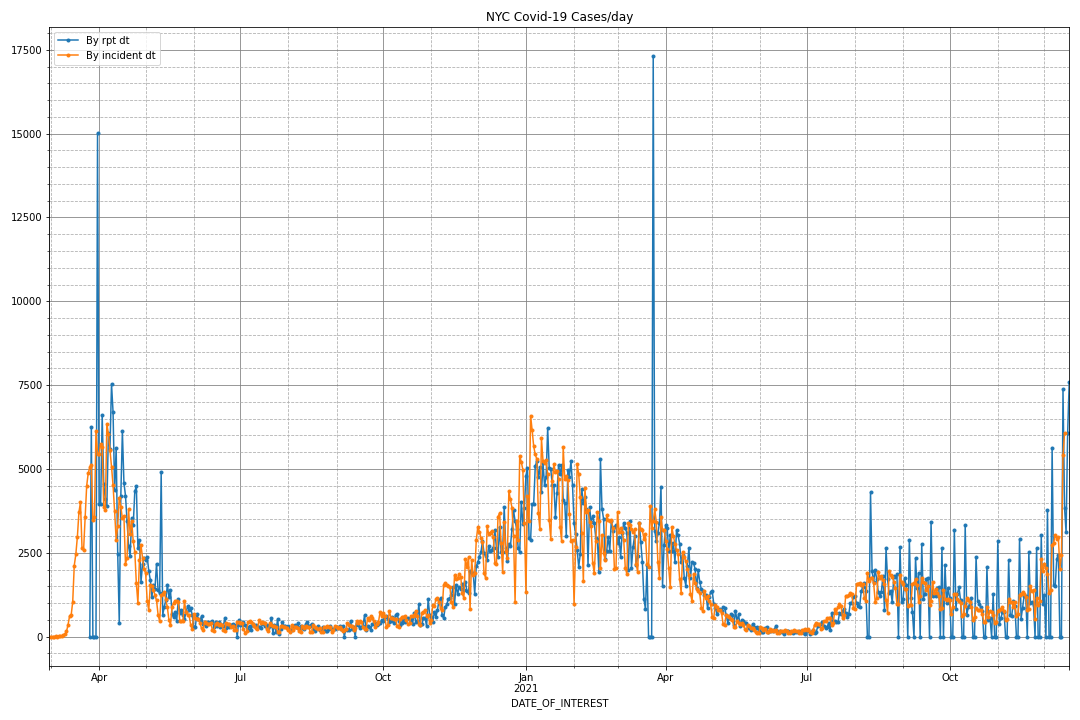
\includegraphics[width=\textwidth]{../Notebooks/casesPerDayHistoryRptDtVsInDtRaw.png}
  \caption{NYC cases per day by incident date vs by reporting date.}
  \label{fig:rptvsdataraw}
\end{figure}

\begin{figure}[H]
  \centering
  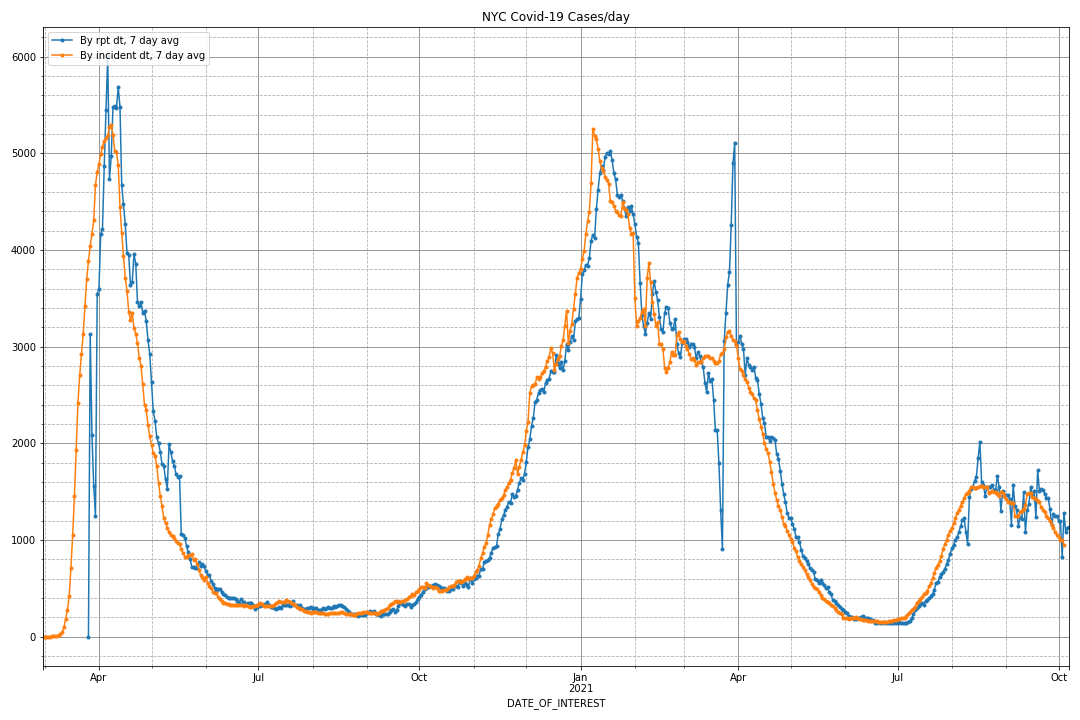
\includegraphics[width=\textwidth]{../Notebooks/casesPerDayHistoryRptDtVsInDt.png}
  \caption{NYC cases per day, 7 day rolling average, by incident date vs by reporting date.}
  \label{fig:rptvsdata7day}
\end{figure}

As you can see, the reporting date data is far noisier; so much so
that the 7 day cycle is obscured and the 7 day rolling window still
shows substantial noise.  For example, the spike on May 11th in the
raw data of about 5,000 cases corresponds to the history being
restated slightly, but going back to the third week of March.  This
gives a substantially distorted view from day to day.  The noise also
makes the peak appear to have occurred much earlier than it actually
does.

The 7 day rolling window shows that the report date data is
overstating the number of cases by a substantial amount, sometimes by
over 50\%.

Surprisingly, the growth rate to the peak is higher rather than lower.
This is presumably because reporting delays were greater when the data
started being collected, leading to batches of reports coming in
together at a later date.

\section{Conclusions}
During this pandemic, it's great to see that organizations like OWID, the
WHO and the ECDC, major news outlets, like The New York Times, and
major universities, like Johns Hopkins University, are all collecting
and aggregating data on COVID-19 cases and deaths and making this data
publicly available.  Without such aggregation, it would be very
difficult to globally understand, analyze, and respond appropriately
to the pandemic.

On the other hand, it's unfortunate that they collect the data in a
way that obscures the current state of the disease and makes analysis
more difficult than it need be.  It's also disturbing that news
agencies are reporting on these numbers as if they actually occurred
on the reporting date, and governments may be taking action based on
the same misconception.

I find it surprising that epidemiologists who make a career out of
analyzing epidemics and pandemics would record the data in such a
fashion.  But, on the other hand, I suppose such work tends to be on a
longer time scale and it's only in the current pandemic that we needed
accurate, up to date infection and death counts.

I'd hope that someone would take it upon themselves to
collect and aggregate the data on an incident date basis.  This would
be a huge undertaking, but the longer this pandemic persists, the more
important this becomes.

\printbibliography

\end{document}
